\section{Architektura}
Rozdział ten opisuje architekturę systemu, zaczynając od najbardziej ogólnego spojrzenia na całość i komunikaty wymieniane pomiędzy poszczególnymi węzłami, kończąc na szczegółowych opisach poszczególnych modułów.






\subsection{Wstęp}
Najmniejsza możliwa konfiguracja systemu to pojedynczy, samodzielnie działający węzeł. Węzeł jest aplikacją Erlang/OTP (z reguły spakowaną razem ze środowiskiem uruchomieniowym przy pomocy reltool'a). W kwestii instalacji i uruchomienia obowiązują więc standardowe procedury.

Węzły są połączone między sobą (znają swoje adresy) w sieć tworzącą graf pełny. Przedstawia to \autoref{fig:arch-overview}. Cała komunikacja między nimi oparta jest wyłącznie na komunikatach języka Erlang. Kiedy nowy węzeł dołączany jest do systemu, pobiera informacje o pozostałych węzłach od jednego z nich, a następnie rozgłasza komunikat o swoim dołączeniu.

\begin{figure}[!htbp]
	\centering
	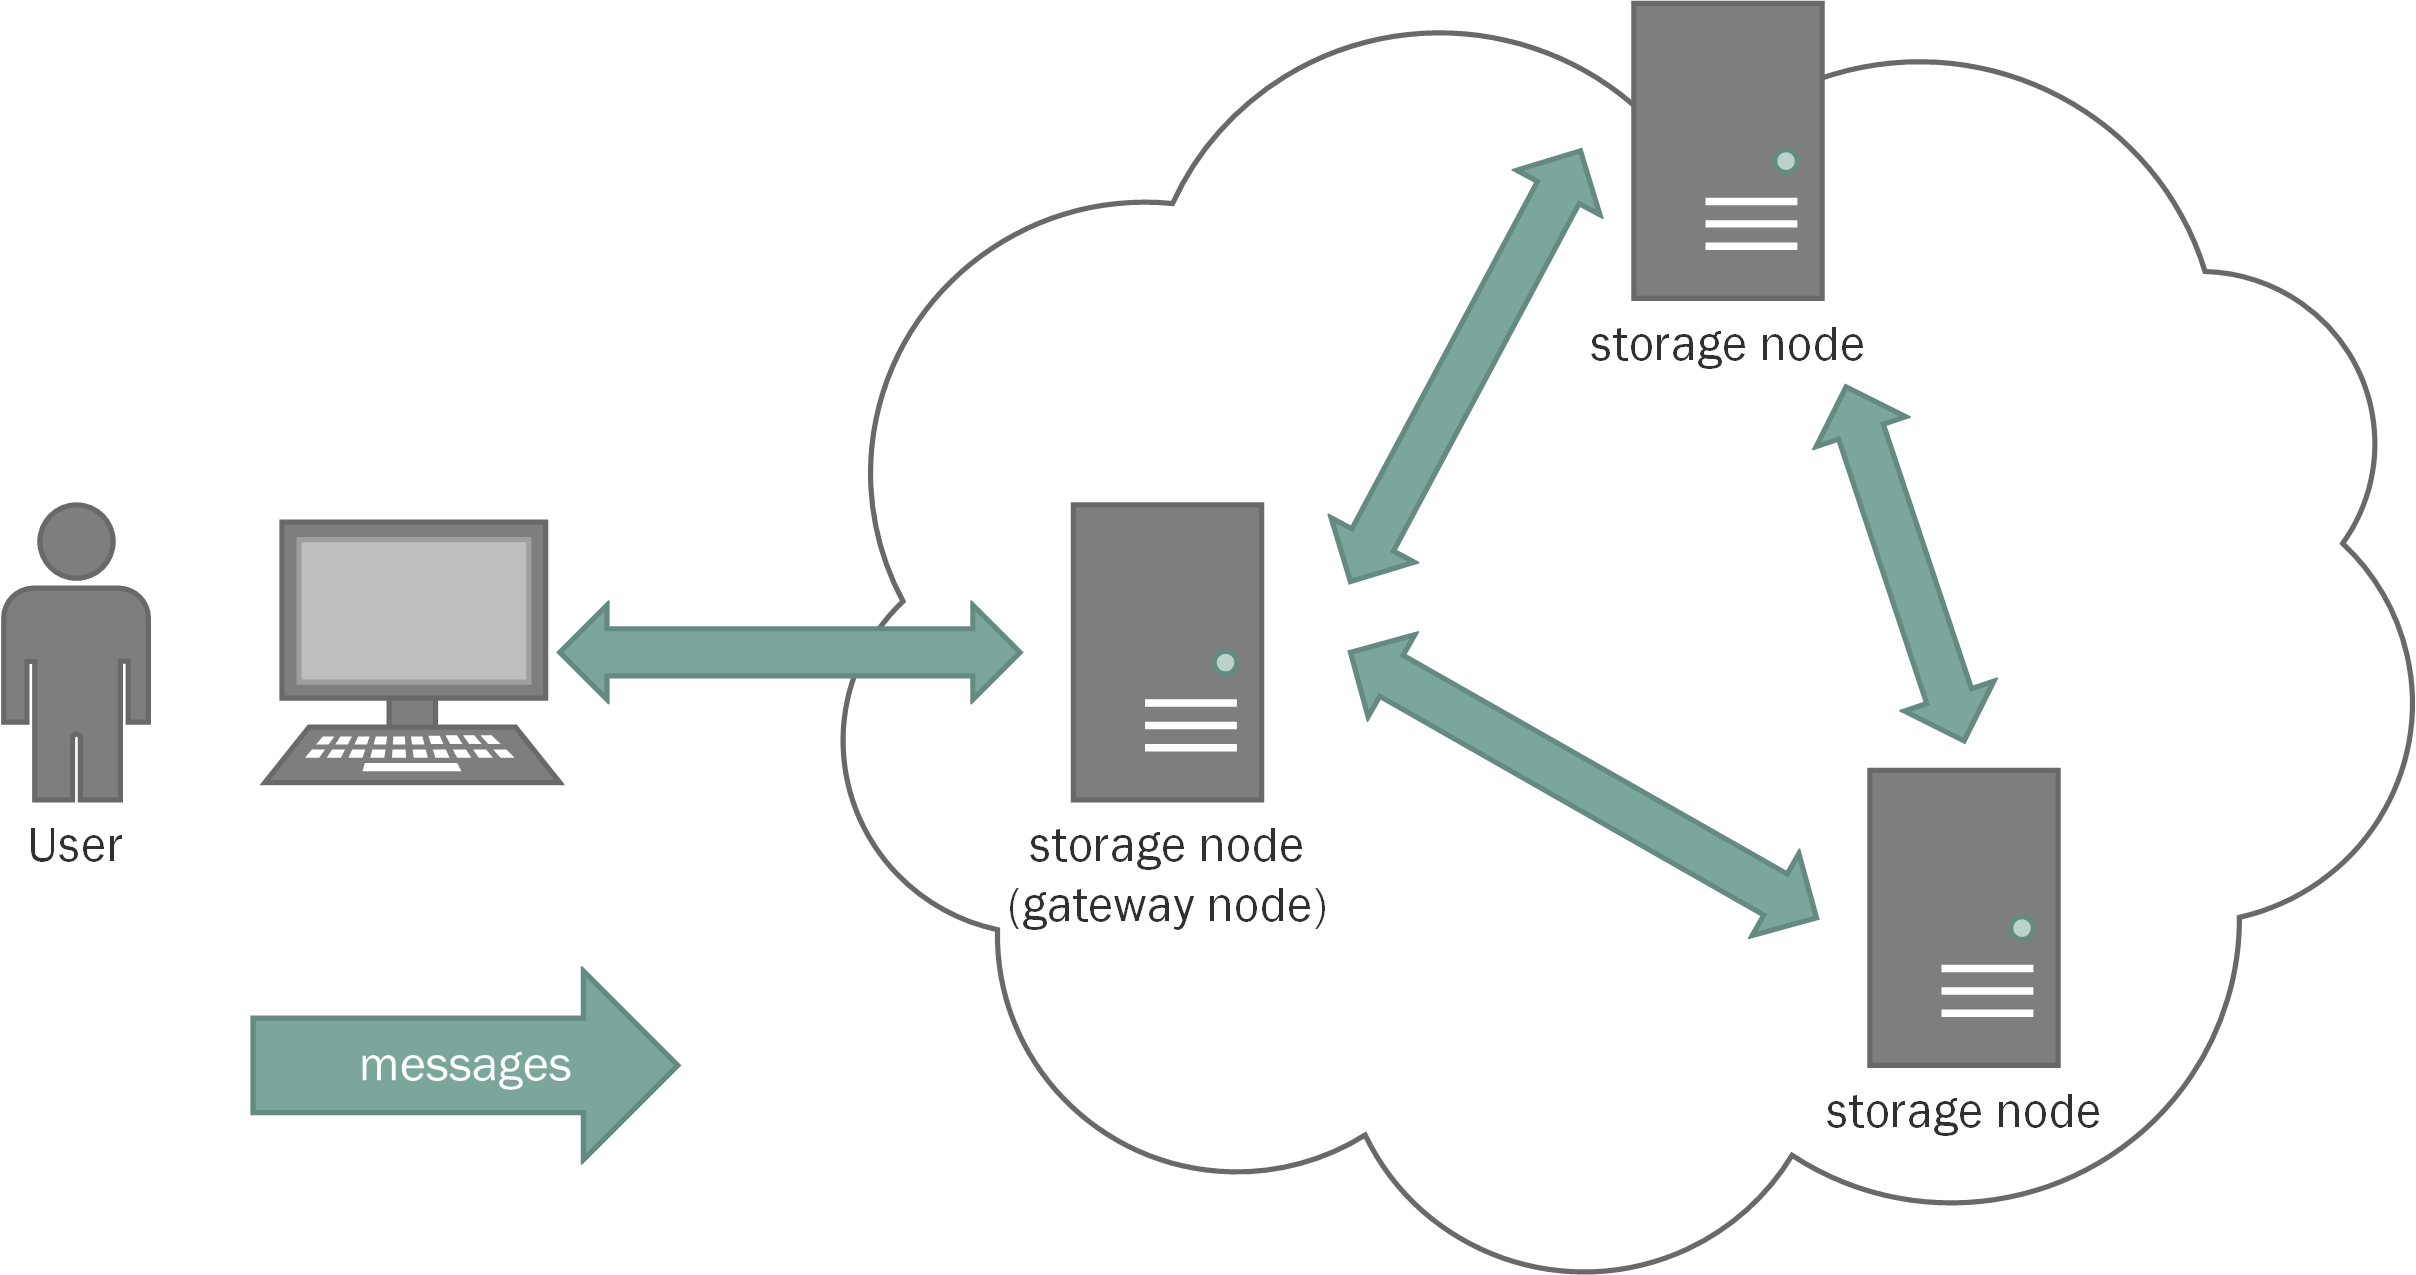
\includegraphics[width=0.8\textwidth]{arch-overview}
	\caption[Diagram architektury systemu.]{System to zdecentralizowana sieć komunikujących się ze sobą węzłów. Komunikaty, w zależności od typu, są rozgłaszane po całym systemie lub kierowane bezpośrednio do odpowiedniego węzła.}
	\label{fig:arch-overview}
\end{figure}

Użytkownik może wykonywać swoje zapytania na dowolnym z węzłów. Zawsze jednak otrzyma dostęp do wszystkich swoich plików, jakie przechowuje w systemie. Wybór węzła dostępowego (gateway node) nie powinien mieć wpływu na wydajność. W związku z tym, że każdy plik może być przechowywany w innym węźle, procedura obsługi zapytań pomija sprawdzanie czy poszukiwany plik znajduje się w aktualnym węźle dostępowym.







\subsection{Struktury}
Spośród wszystkich wymienianych między procesami i węzłami wiadomości, dla trzech z nich zostały zdefiniowane właściwe struktury (rekordy w języku Erlang). Są to struktura użytkownika (User), metadanych pliku (File), zapytania (Request), oraz akcji użytkownika (Action). Pozostałe wiadomości są zwykłymi krotkami zbudowanymi z typów prymitywnych oraz trzech poniżej przedstawianych struktur.

Są to również jedyne obiekty persystowane w bazie danych przy pomocy odpowiednich DAO.

Definicje rekordów znajdują się w pliku storage/include/shared.hrl.

\subsubsection{User}
Definicja rekordu:
\begin{lstlisting}
-record(user, {
	name 		:: nonempty_string(), 
	secret 		:: nonempty_string(), 
	create_time :: integer(), 
}).
\end{lstlisting}

Struktura User reprezentuje użytkownika końcowego systemu. Pola:
\begin{itemize}
	\item name – unikalna nazwa użytkownika / login
	\item secret – prywatny klucz użytkownika używany przy autentykacji
	\item create\_time – data (timestamp) utworzenia konta użytkownika
\end{itemize}

\subsubsection{File}
Definicja rekordu:
\begin{lstlisting}
-record(file, {
	owner 		:: nonempty_string(), 
	vpath 		:: nonempty_string(), 
	bytes 		:: integer(), 
	access_mode :: integer(), 
	create_time :: integer() 
}).
\end{lstlisting}

Struktura File gromadzi metadane dotyczące pliku w systemie. Pola:
\begin{itemize}
	\item owner – identyfikator użytkownika, właściciela pliku
	\item vpath – ścieżka do pliku (UNIX-style). Razem z owner tworzą klucz \item główny listy plików
	\item bytes – rozmiar pliku (w bajtach)
	\item access\_mode – flagi dostępu do pliku
	\item create\_time – data (timestamp) utworzenia pliku
\end{itemize}

\subsubsection{Request}
Definicja rekordu:
\begin{lstlisting}
-record(request, {
	type 				:: 'create' | 'read' | 'update'
						 | 'delete' | 'list' | 'find',
	user 				:: nonempty_string(),
	addr = {none, none} :: { nonempty_string(),
							 nonempty_string() },
	hmac = none 		:: string(), 
	data = none 		:: binary(), 
	opts = none 		:: term() 
}).
\end{lstlisting}

Struktura Request reprezentuje żądanie operacji na pliku. Jest to również podstawowy typ wiadomości w systemie. Przekazywane jest zarówno pomiędzy węzłami jak i wewnątrz węzłów między poszczególnymi modułami. Pola:
\begin{itemize}
	\item type – atom reprezentujący jeden z typów operacji
	\item user – identyfikator użytkownika wykonującego zapytanie
	\item addr - krotka reprezentująca adres żądanego pliku, w postaci \{owner, vpath\}
	\item hmac – suma kontrolna HMAC (więcej w rozdziale dotyczącym autentykacji)
	\item data – binarne dane (w przypadku tworzenia / aktualizacji pliku)
	\item opts – obecnie nie używane
\end{itemize}

\subsubsection{Action}
Definicja rekordu:
\begin{lstlisting}
-record(action, {
	user_id 		:: nonempty_string(), 
	file_id 		, 
	weight 			:: integer(), 
	action_time 	:: integer(), 
	action_type 	:: nonempty_string() 
}).
\end{lstlisting}

Struktura Action tworzona jest przy przetwarzaniu zapytania Request a następnie zapisywana w bazie danych. Lista takich struktur daje opis historii operacji danego użytkownika. Pola:
\begin{itemize}
	\item user\_id – identyfikator użytkownika
	\item file\_id – adres pliku
	\item weight – waga przypisana żądaniu podczas schedulingu
	\item action\_time – data (timestamp) obsługi żądania
	\item action\_type – identycznie jak request\#type, tylko w postaci string()
\end{itemize}





\subsection{Storage}
Pojedynczy węzeł systemu jest aplikacją Erlang/OTP. Składa się z jednego, głównego supervisora zarządzającego pięcioma gen\_serverami: storage\_http\_srv, storage\_auth\_srv, storage\_dist\_srv, storage\_core\_srv oraz storage\_uuid\_srv. storage\_http\_srv jest opcjonalny a jego obecność nie jest wymagana do poprawnej pracy całego systemu. Supervisor pracuje w polityce one-for-one, restartując poszczególne komponenty w razie awarii. Struktura serwerów przedstawiona jest na \autoref{fig:supervision}.

Każdy z gen\_serverów ma jasno określone zadania. Poszczególne serwery (moduły) ściśle współpracują między sobą i wymieniają wiadomości w celu obsługi zapytania. Na podstawie przepływu informacji między nimi można wyróżnić warstwową hierarchię przedstawioną na \autoref{fig:node-overview}. Zapytanie przekazywane jest między kolejnymi modułami:
\begin{enumerate}
	\item storage\_http\_srv (opcjonalnie)
	\item storage\_auth\_srv
	\item storage\_dist\_srv
	\item storage\_core\_srv
\end{enumerate}

Użycie modułu storage\_http\_srv jest opcjonalne – użytkownik może również skorzystać z biblioteki klienckiej (napisanej w Erlangu) i pominąć wysyłanie zapytania przez protokół HTTP.

Szczegółowy opis kolejnych faz obsługi zapytania znajduje się w podrozdziale dotyczącym komunikacji wysokopoziomowej.

\begin{figure}[!htbp]
	\centering
	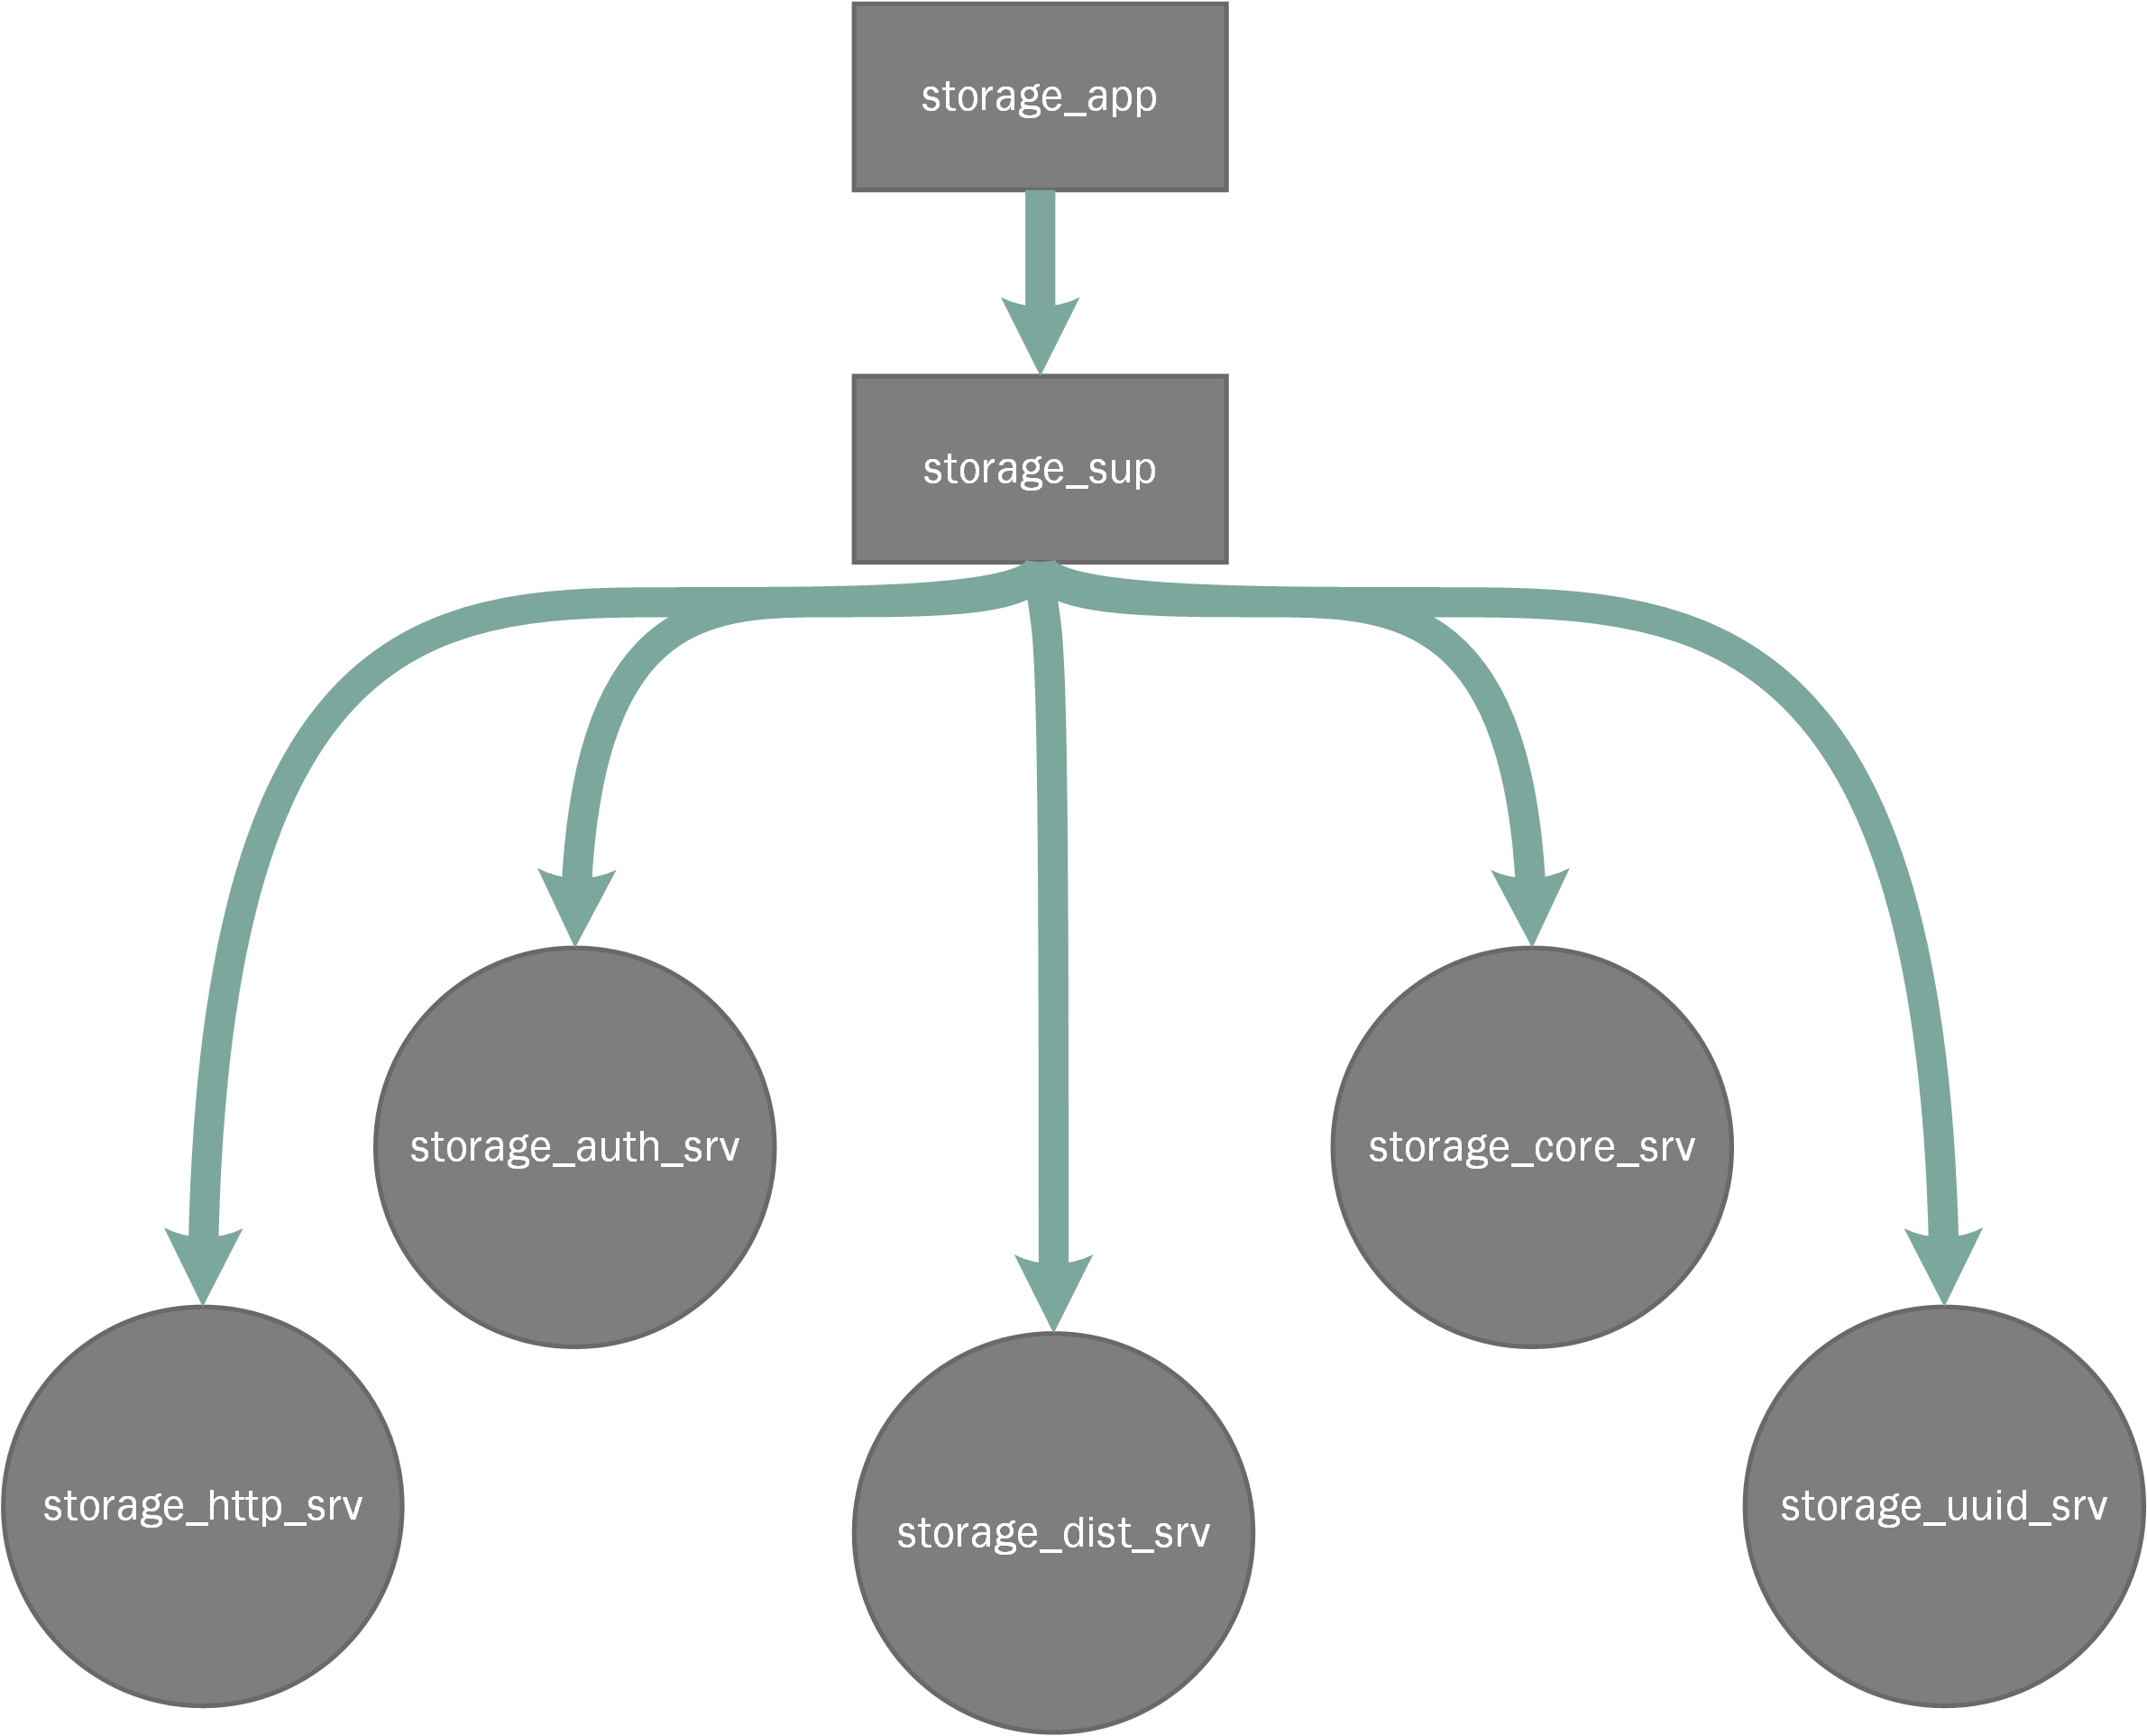
\includegraphics[width=0.8\textwidth]{supervision}
	\caption[Supervision tree.]{Supervision tree. Aplikacja zbudowana jest z pięciu gen\_serverów. Każdy jest osobnym procesem. Ponadto storage\_core\_srv zarządza pulą procesów wykonawczych.}
	\label{fig:supervision}
\end{figure}

\begin{figure}[!htbp]
	\centering
	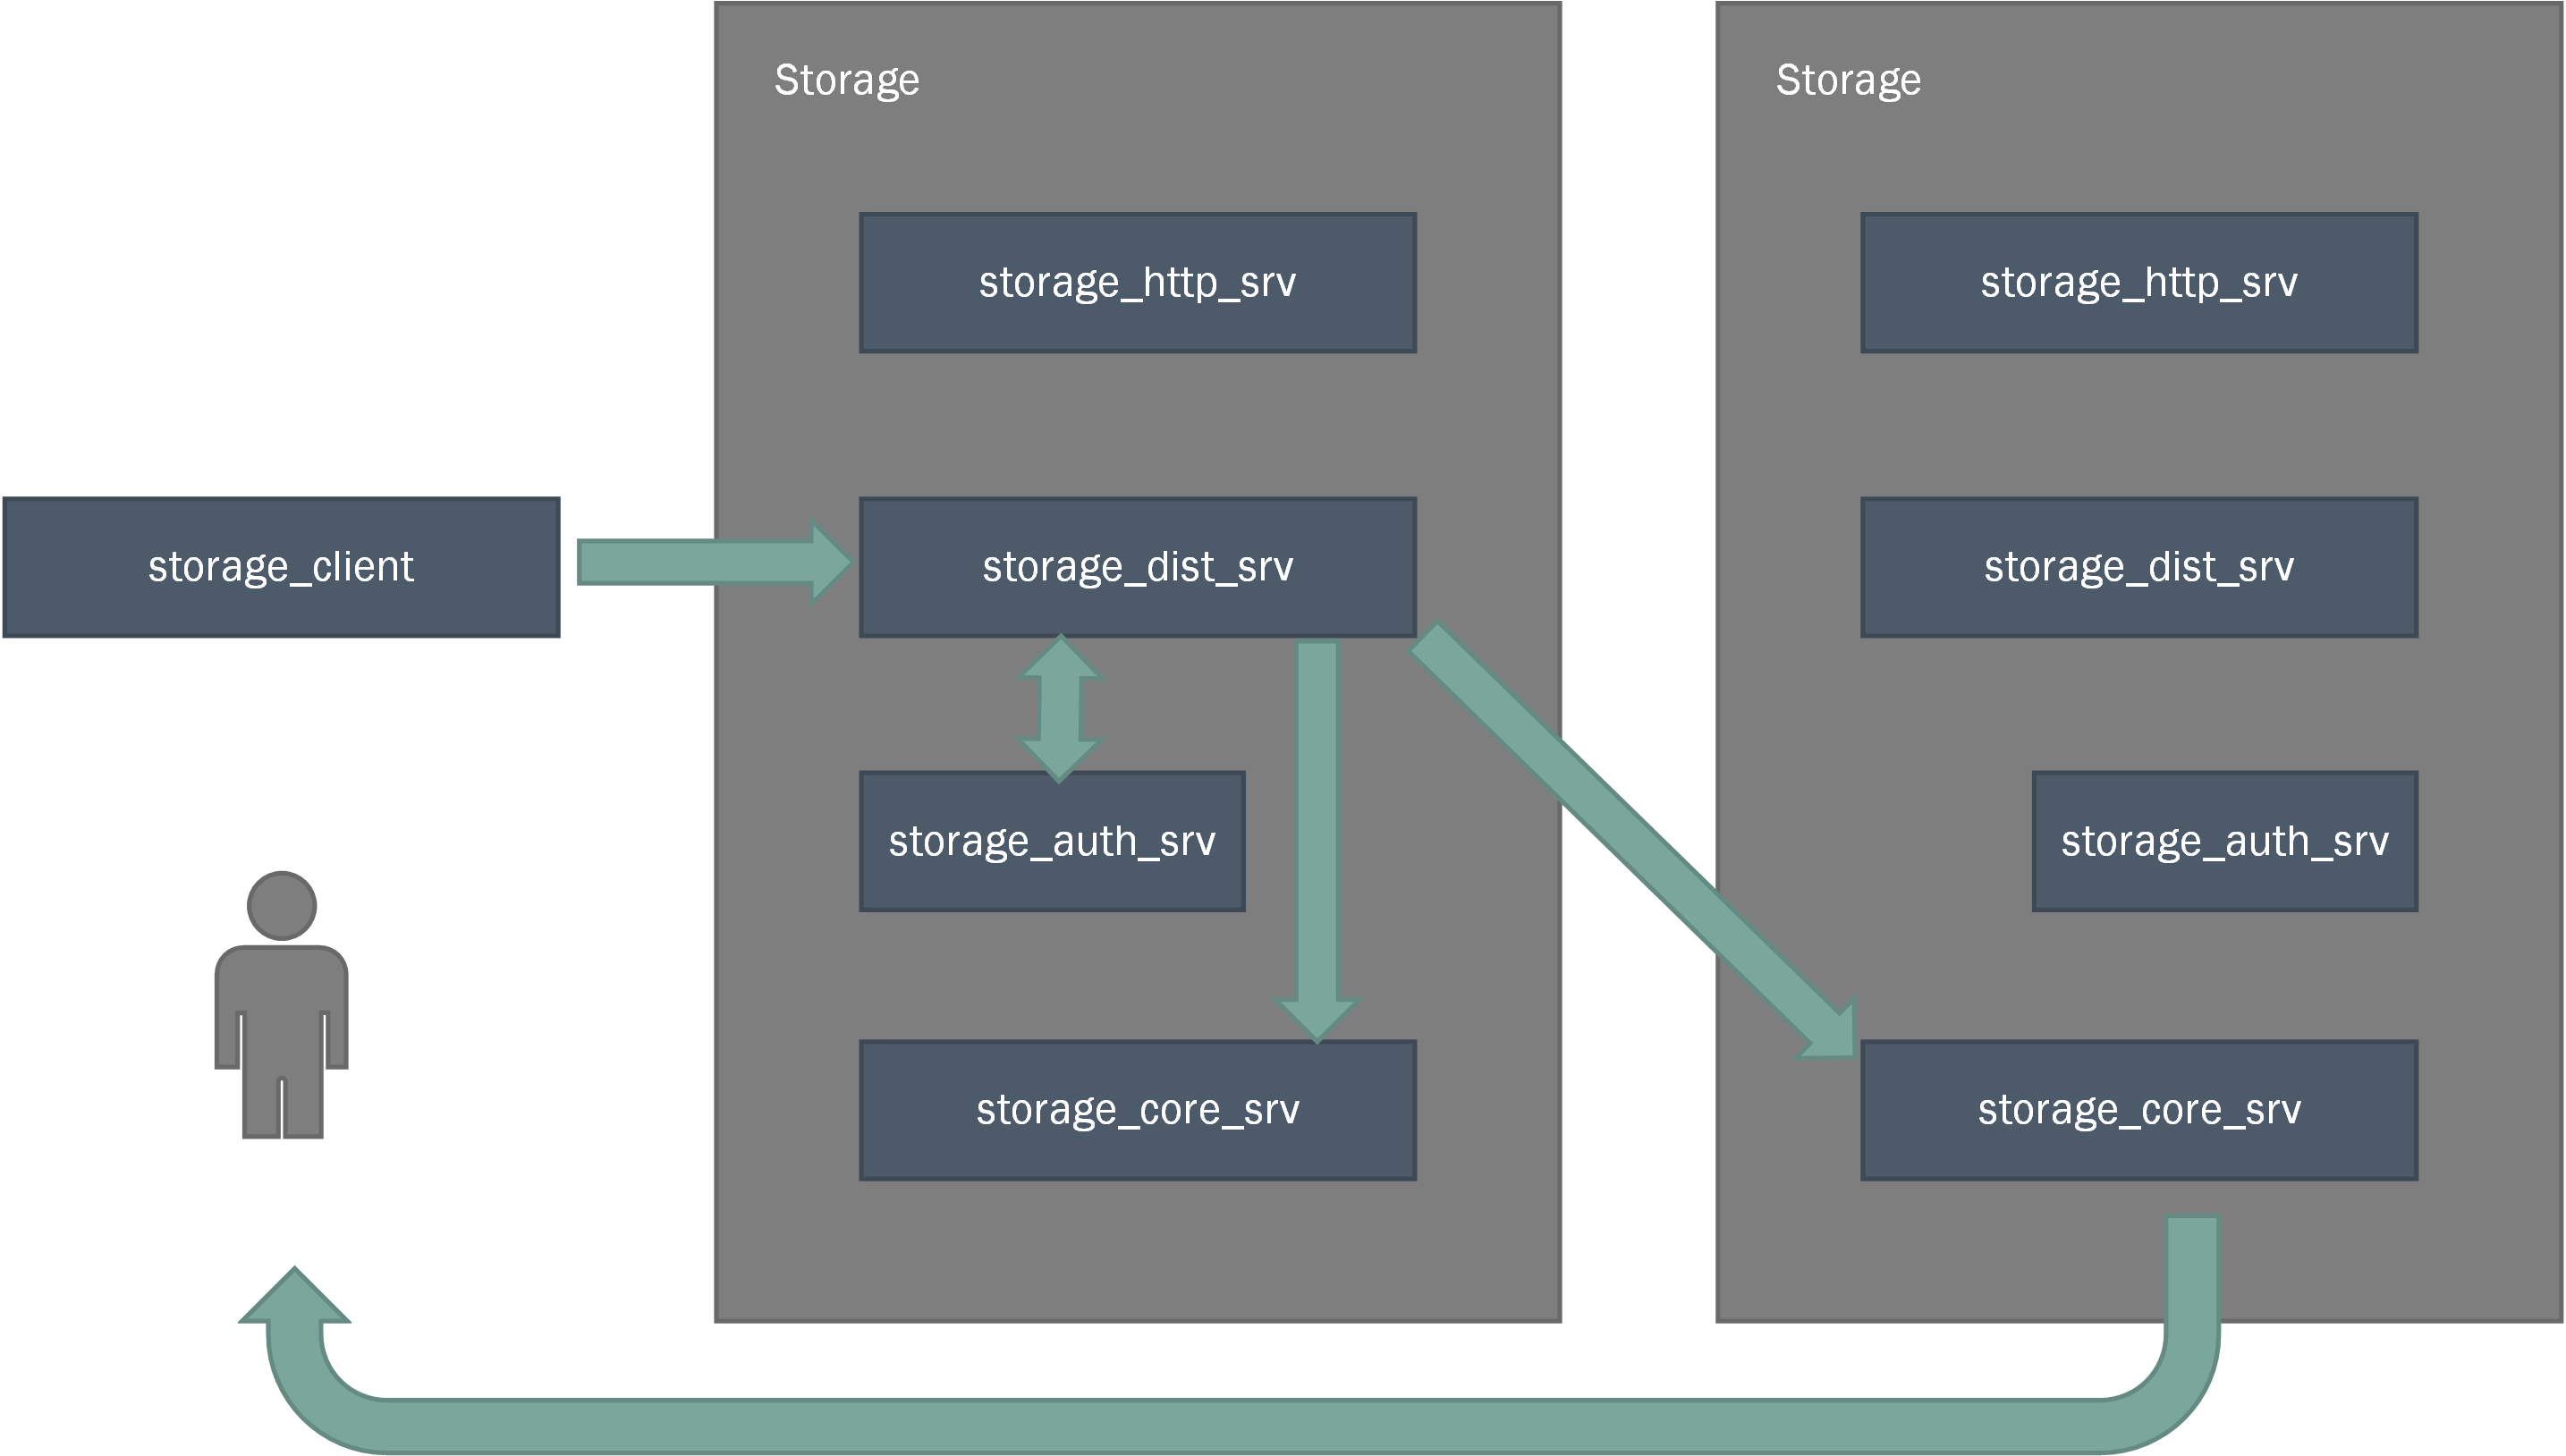
\includegraphics[width=0.8\textwidth]{node-overview}
	\caption[Przepływ zapytania w systemie.]{Przepływ zapytania w systemie. Zapytanie jest rozgłaszane do wszystkich węzłów. Zielone linie oznaczają przepływ zapytania.}
	\label{fig:node-overview}
\end{figure}

\subsubsection{Komunikacja wysokopoziomowa}
Komunikacja pomiędzy węzłami oparta jest w całości na przesyłaniu struktur Request. W zależności od typu zapytania, w procedurze obsługi występują nieznaczne różnice. Można jednak przedstawić to w postaci listy modułów, gdzie kolejno trafia zapytanie:

\begin{enumerate}
	\item (opcjonalnie) storage\_http\_srv – zapytanie jest parsowane, tworzona jest struktura Request
	\item storage\_dist\_srv – przyjmuje strukturę Request, przekazuje do autentykacji
	\item storage\_auth\_srv – autentykuje i sprawdza spójność przekazanego zapytania
	\item storage\_dist\_srv
	\begin{enumerate}
		\item zapytania create / update – wyszukuje odpowiedni węzeł i przekazuje strukturę Request do działającego na nim storage\_core\_srv
		\item pozostałe zapytania – rozgłasza strukturę Request do serwerów storge\_core\_srv na wszystkich węzłach w systemie
	\end{enumerate}
	\item storage\_core\_srv – dokonuje obsługi zapytania lub odrzuca je, jeżeli dotyczy pliku który nie znajduje się w danym węźle. Odpowiedź kierowana jest prosto do użytkownika
\end{enumerate}

\begin{figure}[!htbp]
	\centering
	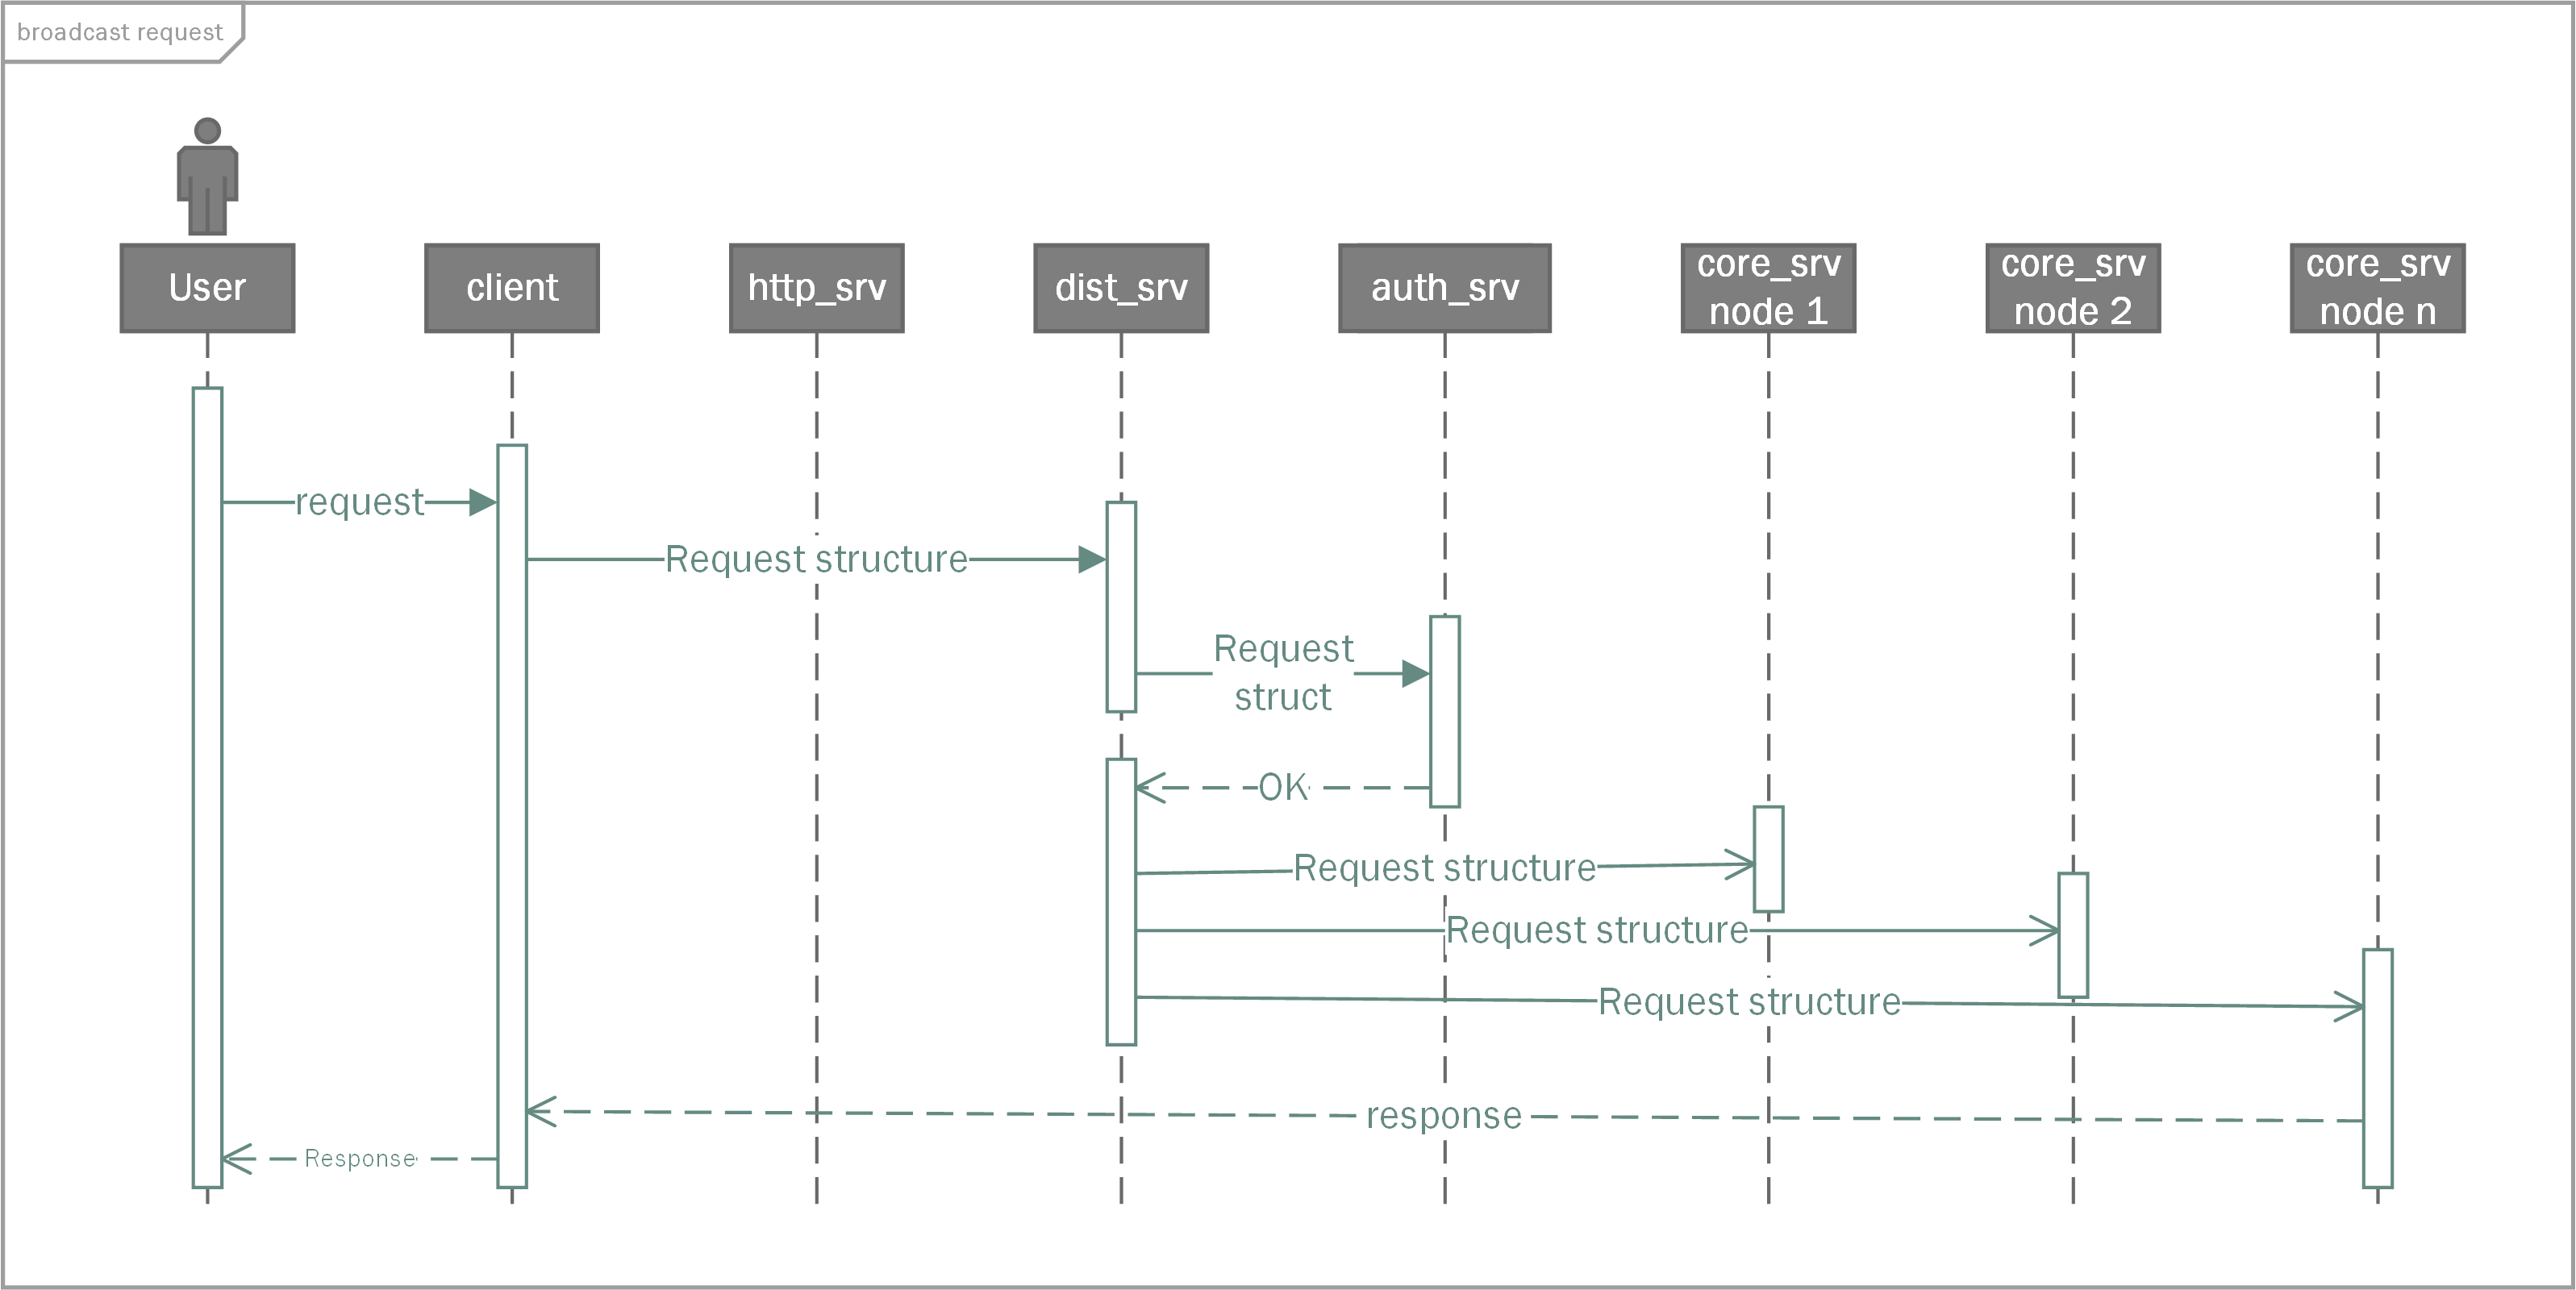
\includegraphics[width=0.9\textwidth]{broadcast-seq}
	\caption[Zapytanie rozgłoszeniowe (Erlang).]{Zapytanie rozgłoszeniowe z wykorzystaniem biblioteki klienckiej zakończone powodzeniem.}
	\label{fig:broadcast-seq}
\end{figure}

\autoref{fig:broadcast-seq} pokazuje diagram sekwencji obsługi zapytań rozgłoszeniowych z wykorzystaniem biblioteki klienckiej. Zapytania tego typu to zapytania read, delete oraz find. \autoref{fig:broadcast-http-seq} pokazuje te same akcje przy wykorzystaniu modułu HTTP. Widać, że moduł HTTP wewnętrznie korzysta z biblioteki klienckiej. Rysunki zakładają, że autentykacja przebiegła pomyślnie a jeden z węzłów zawierał żądany plik. Użytkownikowi odpowiada tylko jeden węzeł - ten, który obsłużył zapytanie (przechowywał poszukiwany plik). Pozostałe węzły ignorują komunikat.

\begin{figure}[!htbp]
	\centering
	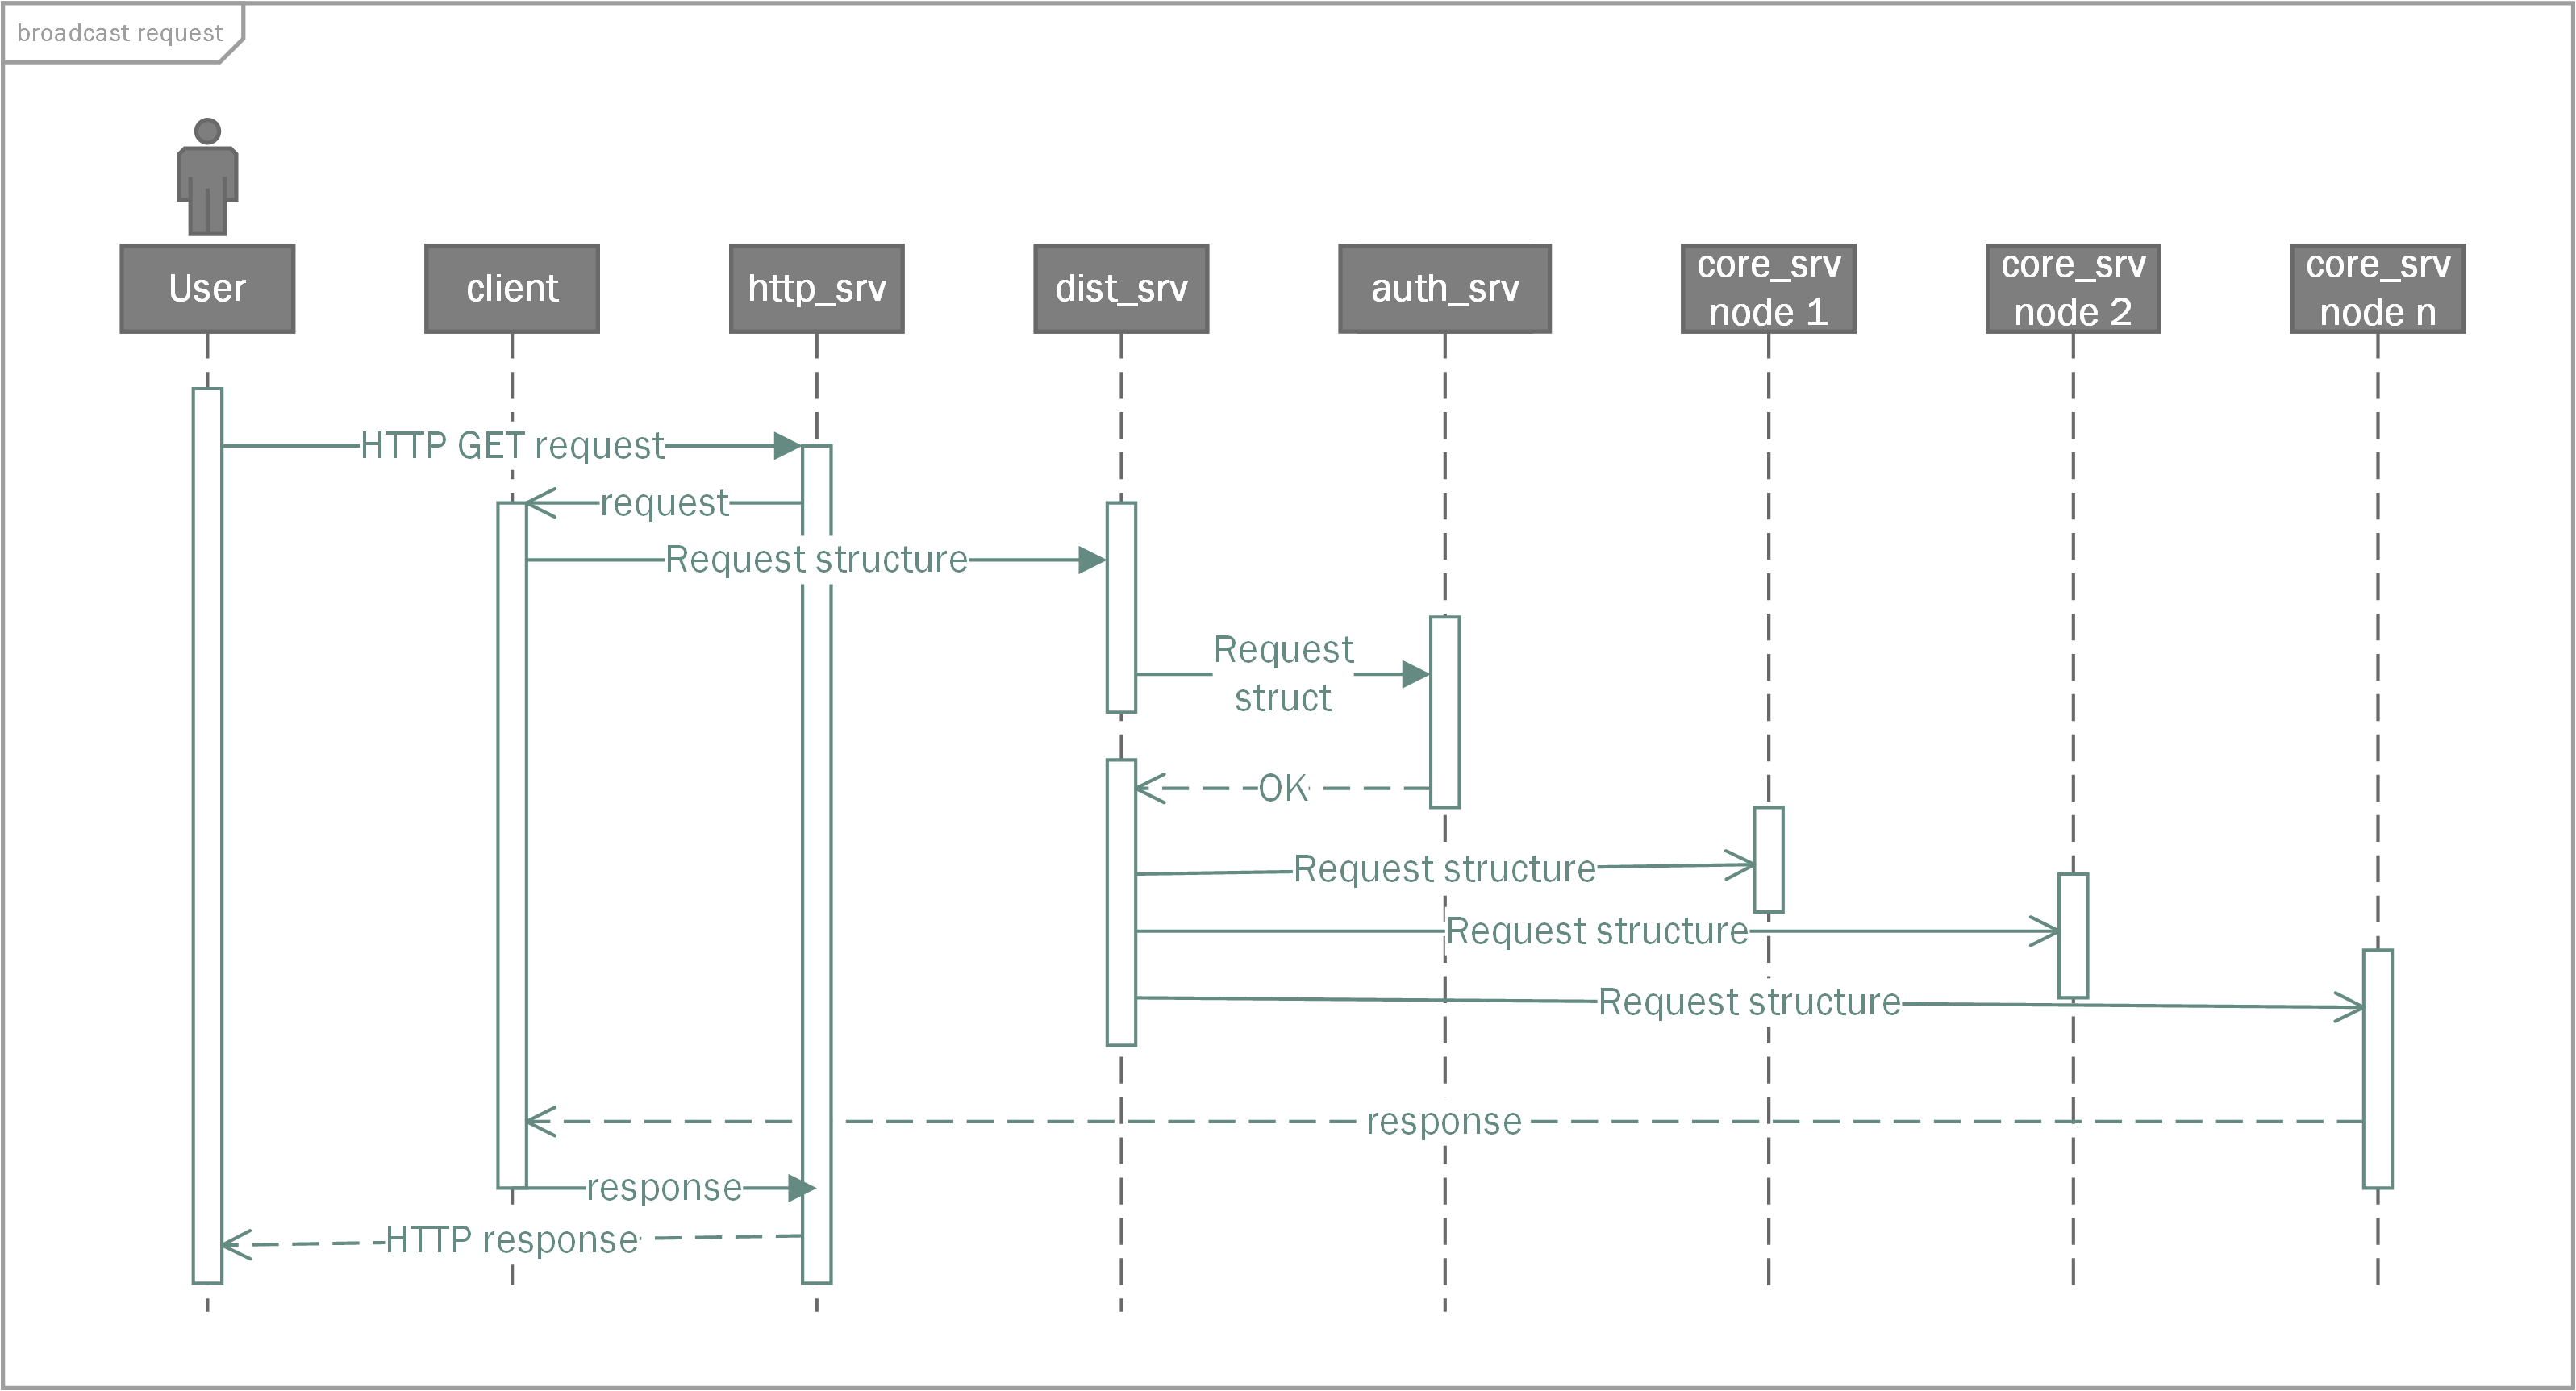
\includegraphics[width=0.9\textwidth]{broadcast-http-seq}
	\caption[Zapytanie rozgłoszeniowe (HTTP).]{Zapytanie rozgłoszeniowe z wykorzystaniem modułu HTTP. Użytkownik wysyła zapytanie metodą GET, które tłumaczone jest na odpowiednią strukturę Request.}
	\label{fig:broadcast-http-seq}
\end{figure}

Zapytania typu create i update nie są rozgłaszane. Najbardziej odpowiedni na przyjęcie nowych danych węzeł jest wybierany spośród wszystkich węzłów w systemie. Wybór ten dokonywany jest w węźle, do którego początkowo trafia zapytanie (gateway node). Jedyną różnicą w stosunku do \autoref{fig:broadcast-seq} oraz \autoref{fig:broadcast-http-seq} byłoby zaznaczenie pojedynczego modułu core\_srv, działającego na docelowym węźle.

W przypadku zapytania o listę wszystkich plików (zapytanie list), przeszukane muszą zostać wszystkie węzły. Odpowiedź nie wraca jednak z każdego z nich bezpośrednio do klienta, lecz do modułu dist\_srv, odpowiedzialnego za połączenie wszystkich list w jedną listę wynikową. Sytuację tę przedstawia diagram na \autoref{fig:broadcast-list}.

\begin{figure}[!htbp]
	\centering
	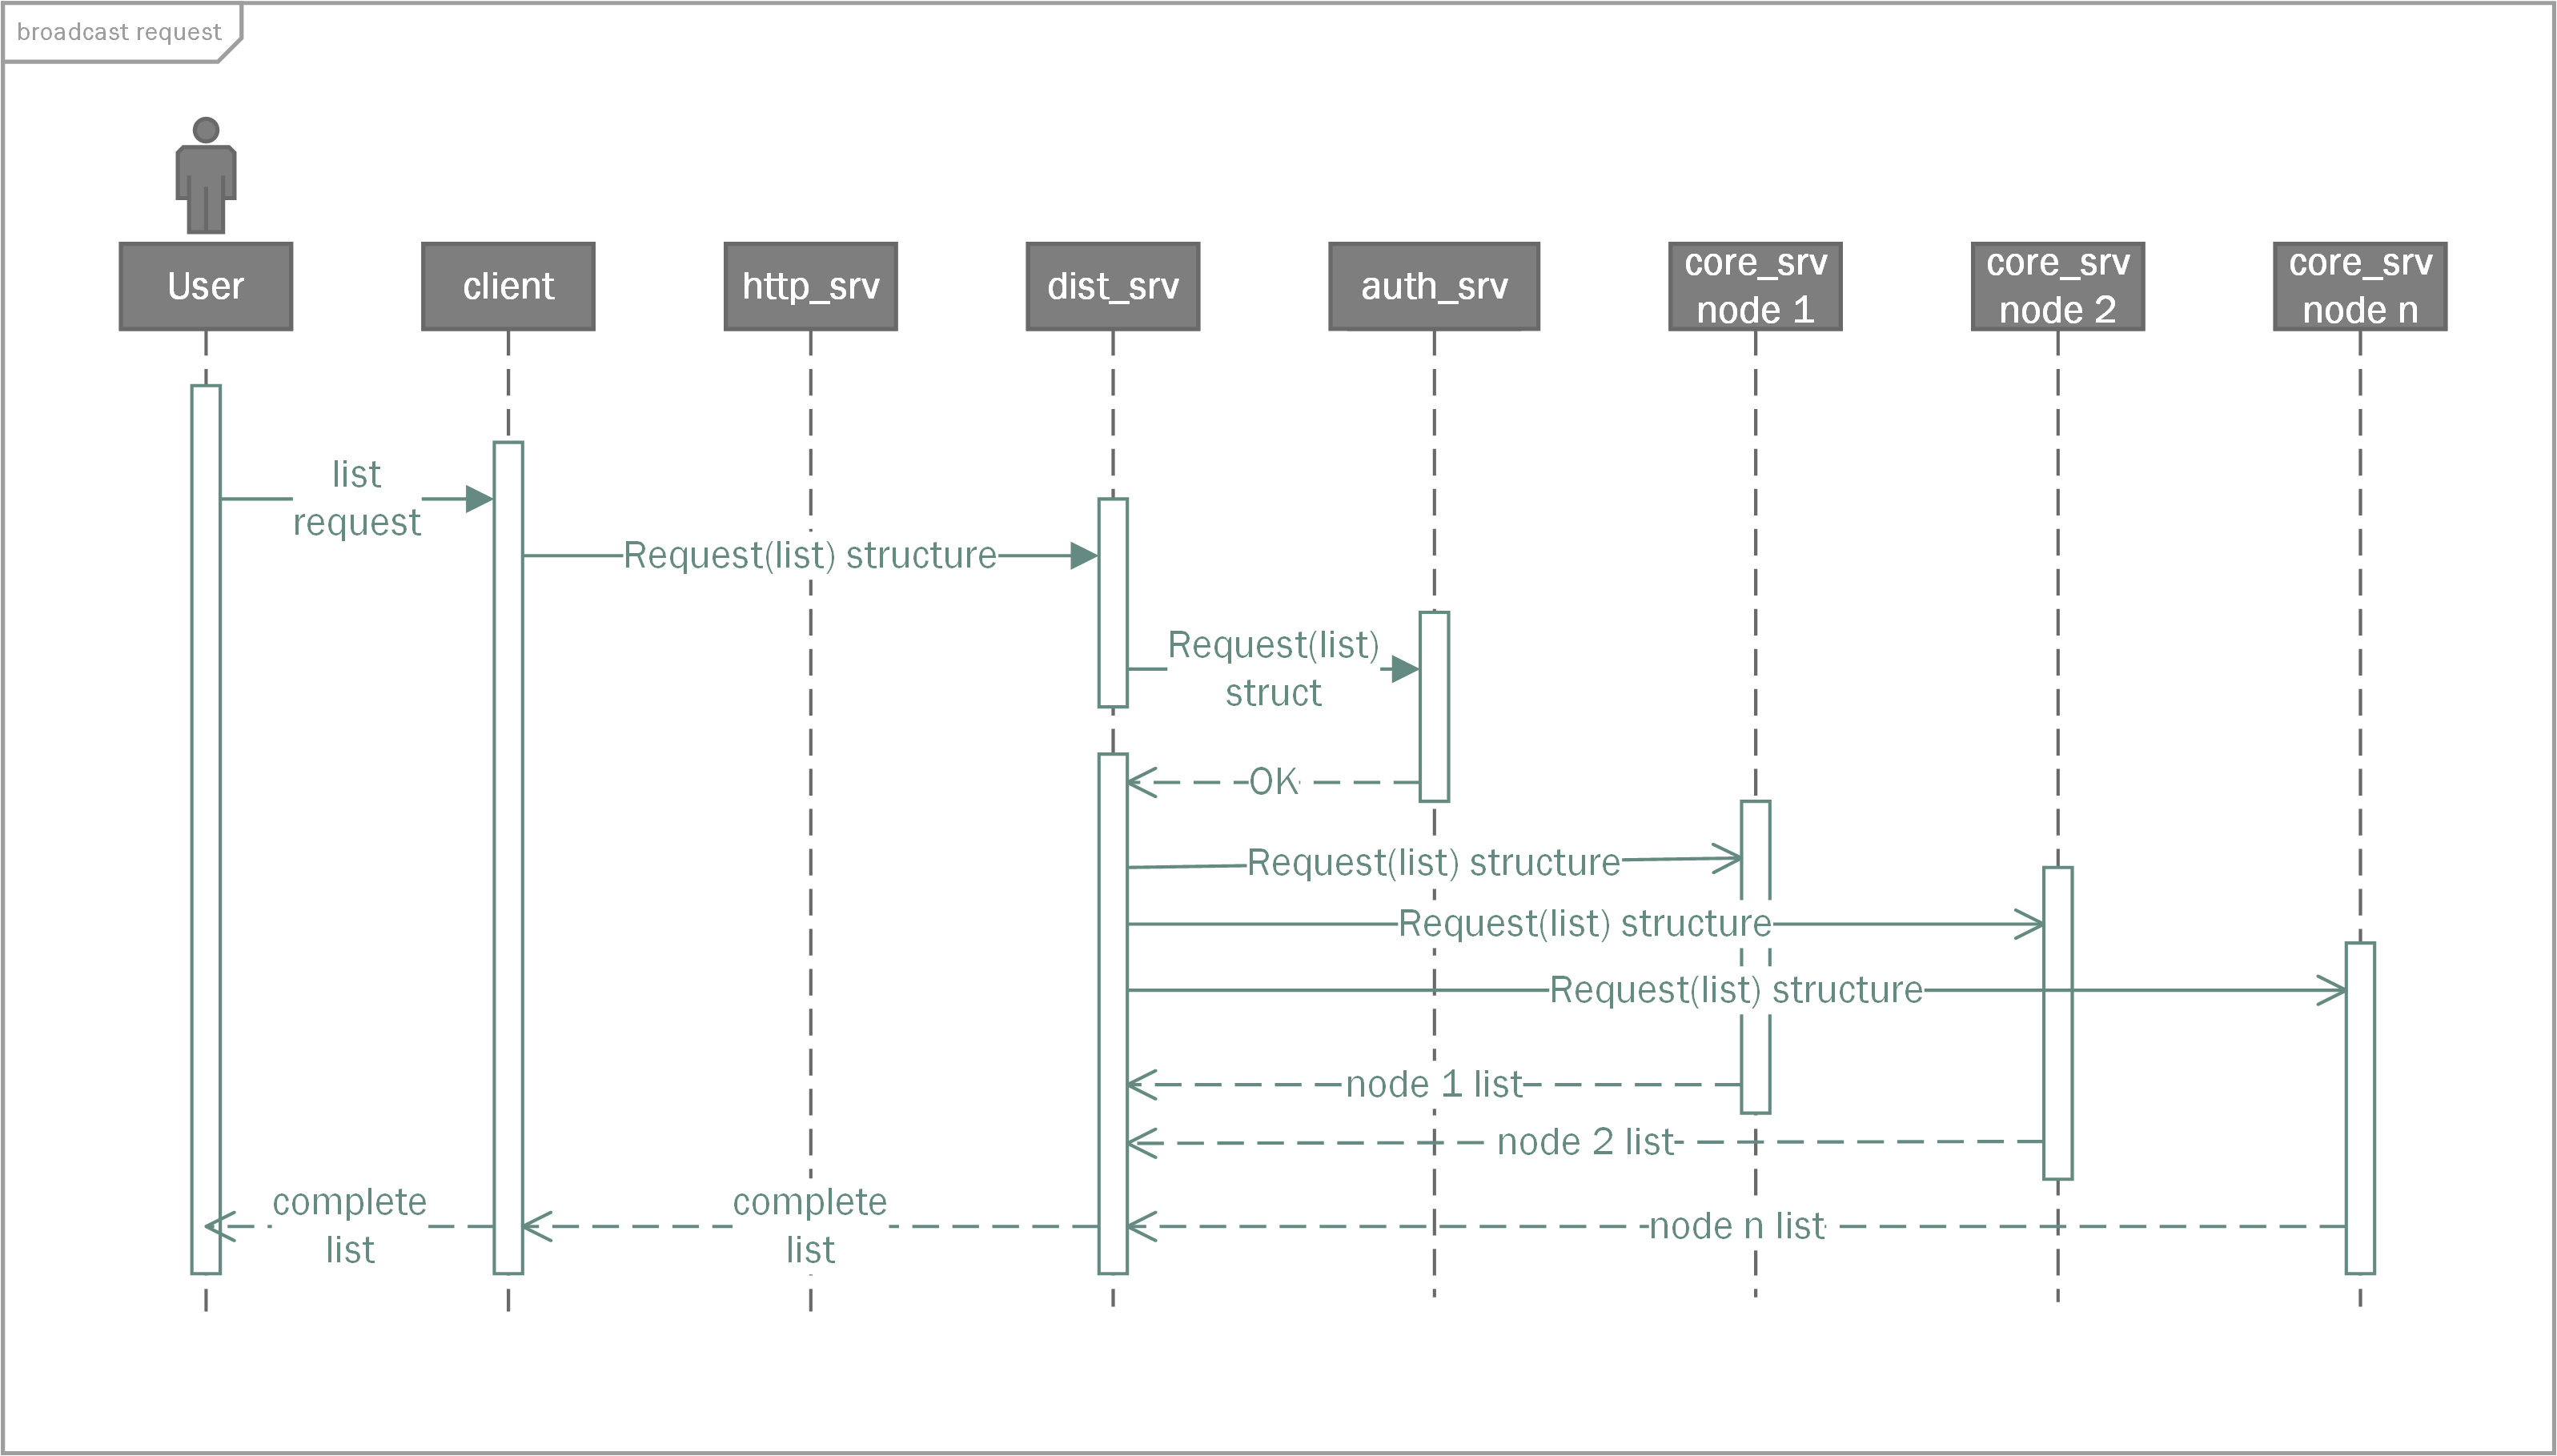
\includegraphics[width=0.9\textwidth]{broadcast-list}
	\caption[Zapytanie o listę plików.]{Obsługa zapytania o listę wszystkich plików użytkownika.}
	\label{fig:broadcast-list}
\end{figure}

\subsubsection{Obsługa błędnych zapytań}
Istnieją sytuacje, kiedy żądanie przesłane do systemu kończy się niepowodzeniem – kiedy nie udało się znaleźć pliku który użytkownik chciał odczytać lub w systemie nie ma miejsca na stworzenie nowego pliku. Można rozróżnić tutaj dwa scenariusze: system od razu sygnalizuje błąd oraz system 'zawiesza się', w oczekiwaniu na odpowiedź jednego z węzłów. 

Pierwszy ma miejsce w przypadki zapytań create i update, kiedy moduł storage\_dist\_srv zwraca do biblioteki klienckiej błąd o niemożliwości zapisania pliku. Wszystkie pozostałe zapytania (zapytania rozgłoszeniowe) mają ustalony pewien czas (domyślnie 10 sekund), po którym jeżeli biblioteka kliencka nie otrzyma odpowiedzi, zgłasza błąd. Taki scenariusz przedstawia \autoref{fig:broadcast-error}.

\begin{figure}[!htbp]
	\centering
	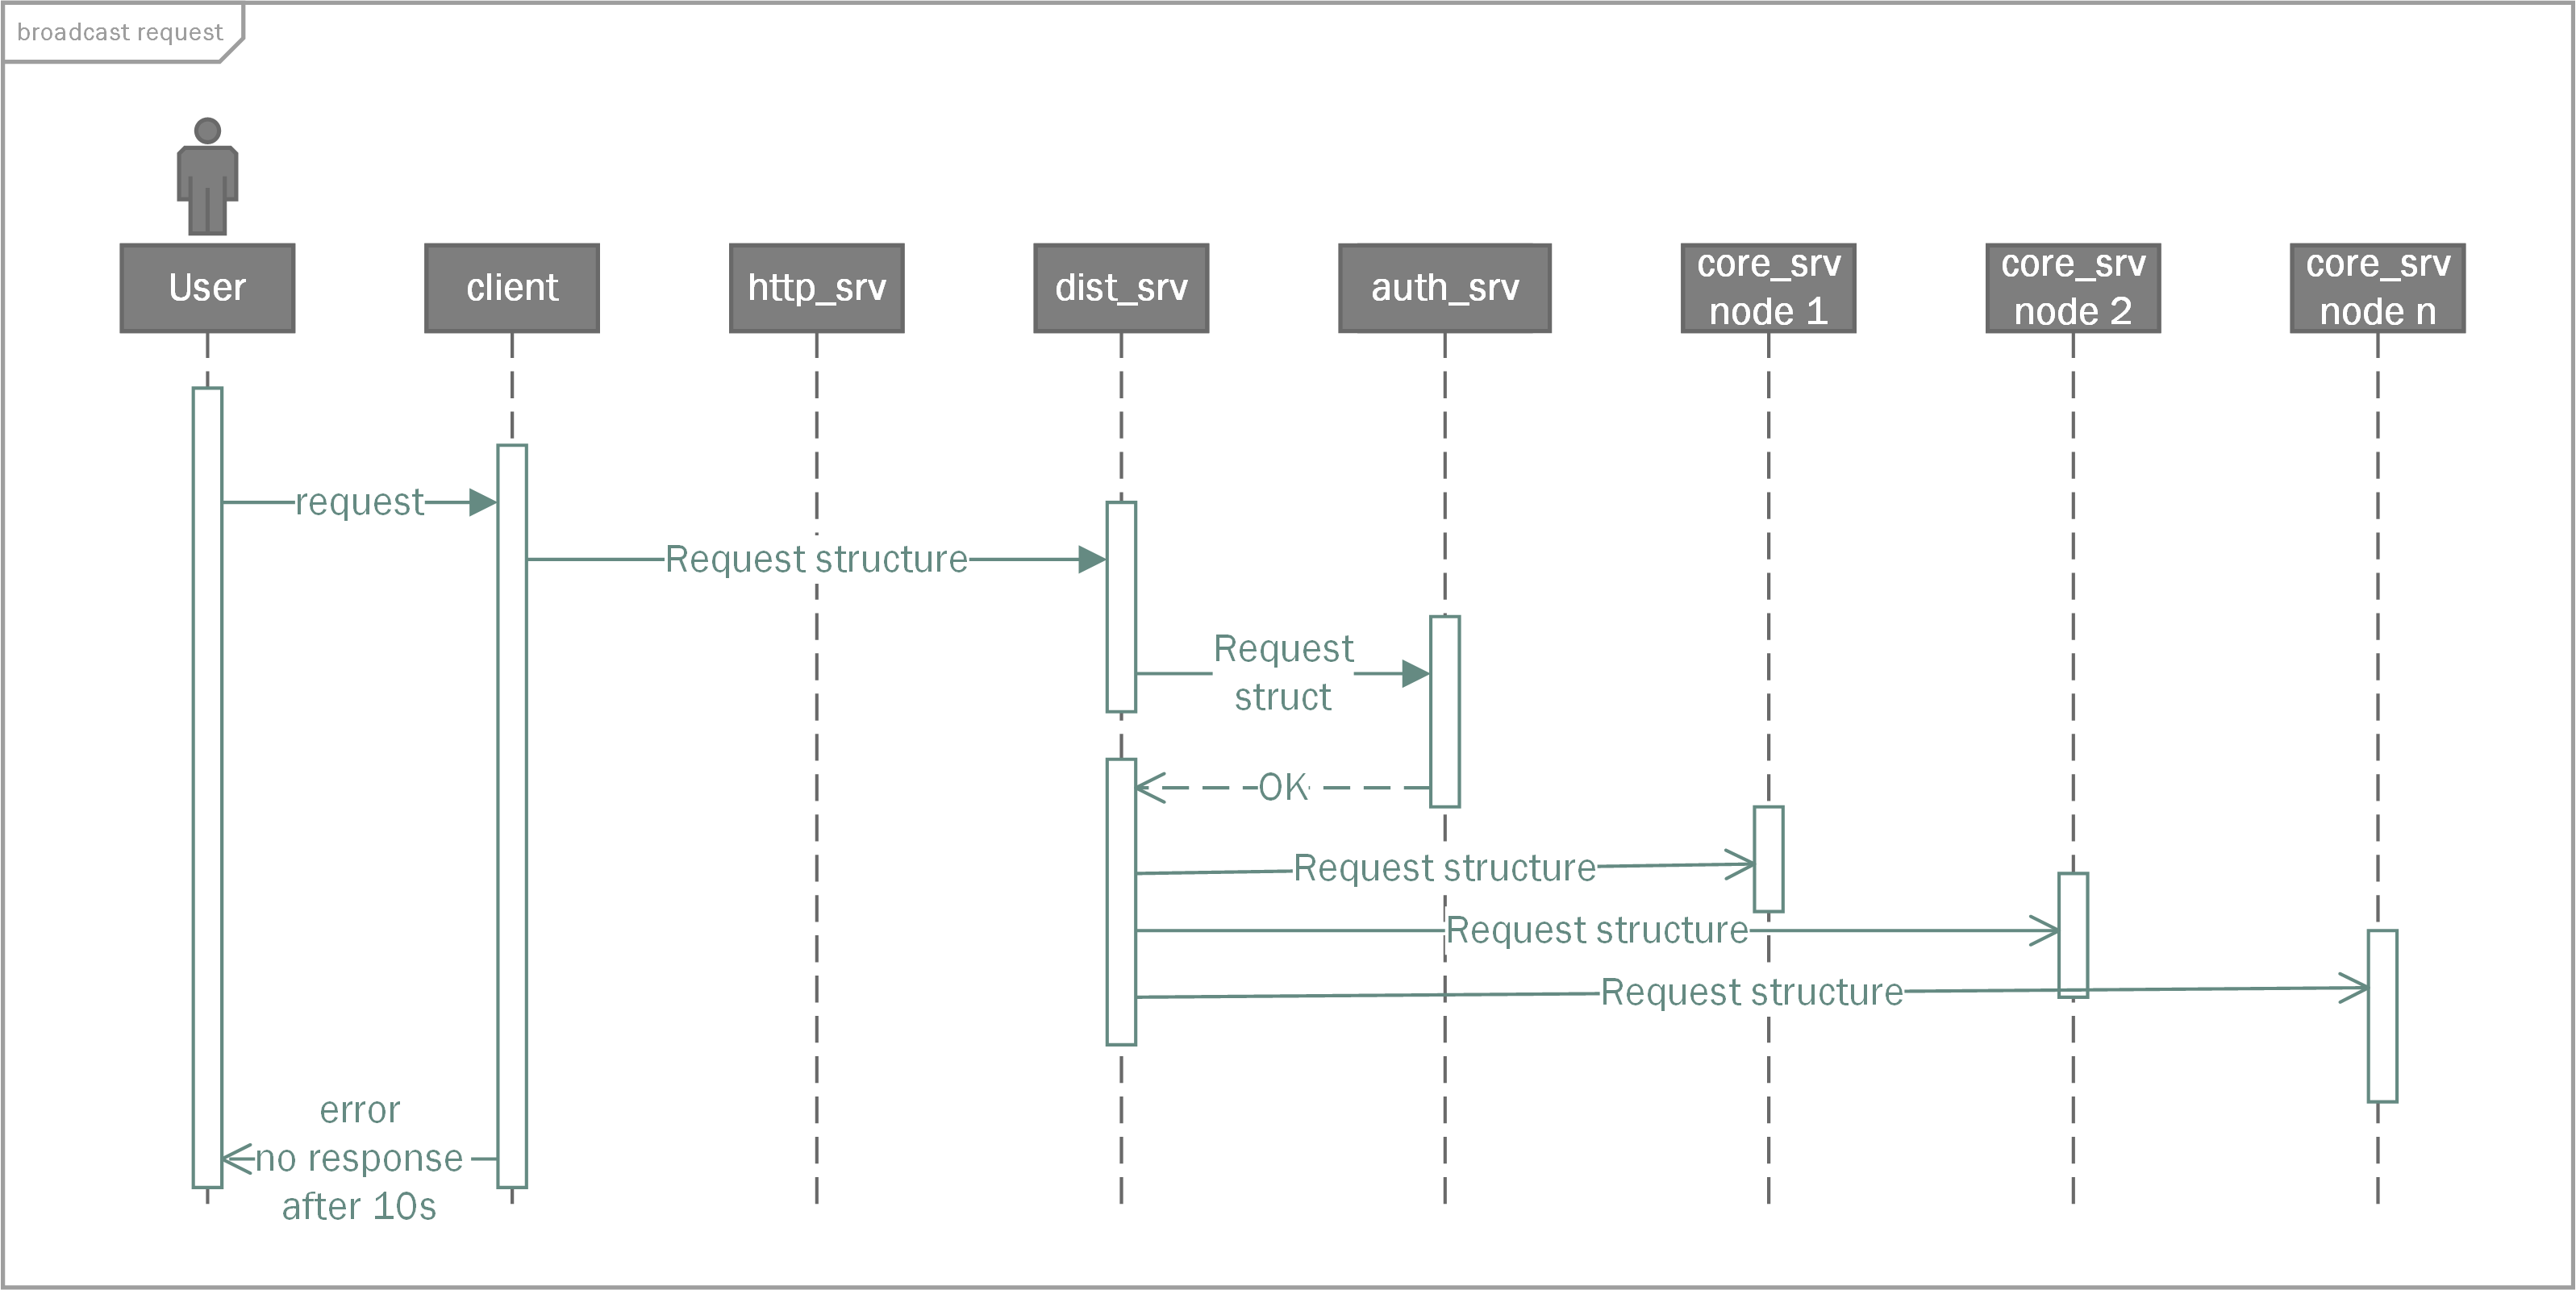
\includegraphics[width=0.9\textwidth]{broadcast-error}
	\caption[Zapytanie zakończone błędem.]{Zapytanie rozgłoszeniowe zakończone niepowodzeniem. Jeżeli biblioteka kliencka nie otrzyma przez pewien czas odpowiedzi z żadnego z węzłów, zakłada się że poszukiwany plik nie istnieje (węzeł który nie posiada szukanego pliku ignoruje zapytania).}
	\label{fig:broadcast-error}
\end{figure}